\documentclass[letterpaper,11pt]{article}
\oddsidemargin -1.0cm \textwidth 17.5cm

\usepackage[utf8]{inputenc}
\usepackage[activeacute,spanish, es-lcroman]{babel}
\decimalpoint
\usepackage{amsfonts,setspace}
\usepackage{amsmath}
\usepackage{amssymb, amsmath, amsthm}
\usepackage{comment}
\usepackage{float}
\usepackage{amssymb}
\usepackage{dsfont}
\usepackage{anysize}
\usepackage{multicol}
\usepackage{enumerate}
\usepackage{graphicx}
\usepackage[left=1.5cm,top=2cm,right=1.5cm, bottom=1.7cm]{geometry}
\setlength\headheight{1.5em} 
\usepackage{fancyhdr}
\usepackage{multicol}
\usepackage{hyperref}
\usepackage{wrapfig}
\usepackage{subcaption}
\usepackage{siunitx}
\usepackage{cancel}
\pagestyle{fancy}
\fancyhf{}
\renewcommand{\labelenumi}{\normalsize\bfseries P\arabic{enumi}.}
\renewcommand{\labelenumii}{\normalsize\bfseries (\alph{enumii})}
\renewcommand{\labelenumiii}{\normalsize\bfseries \roman{enumiii})}


\begin{document}

\fancyhead[L]{\itshape{Facultad de Ciencias F\'isicas y Matem\'aticas}}
\fancyhead[R]{\itshape{Universidad de Chile}}

\begin{minipage}{11.5cm}
    \begin{flushleft}
        \hspace*{-0.6cm}\textbf{FI1000-6 Introducción a la Física Clásica}\\
        \hspace*{-0.6cm}\textbf{Profesora:} Paulina Lira\\
        \hspace*{-0.6cm}\textbf{Auxiliares:} Juan Cristóbal Castro \& Alejandro Silva\\
        \hspace*{-0.6cm}\textbf{Ayudantes:} Francisca Bórquez, Catalina Molina \& Erick Pérez\\
        
    \end{flushleft}
\end{minipage}

\begin{picture}(2,3)
    \put(366, 10){
\includegraphics[scale=0.9]{2020-1/Imágenes/logo/dfi-fcfm.pdf}}
\end{picture}

\begin{center}
	\LARGE\textbf{Auxiliar \#2}\\
	\Large{Caída libre y lanzamiento de proyectil}
\end{center}

\vspace{-1cm}
\begin{enumerate}\setlength{\itemsep}{0.4cm}

\rfoot[]{pág. \thepage}

\item[]

\item Un cohete se dispara verticalmente, subiendo con una aceleración constante $a_0$ respecto a la plataforma de lanzamiento durante un tiempo $\tau$. En ese momento se agota su combustible y continua moviéndose bajo la acción de la aceleración de gravedad.
    \begin{enumerate}
        \item ¿Cuál es la máxima altura que alcanza?
        \item ¿Cuál es el tiempo transcurrido desde que despega hasta volver a caer sobre la plataforma?
    \end{enumerate}
    
\item Un volcán eyecta lava y rocas desde su cráter. Suponga que una roca es eyectada con una velocidad inicial de $v_0 = $ \SI{25}{\m/\s} a un ángulo de $\theta = $ $35^{\circ}$ con respecto a la horizontal como lo muestra la figura. La roca impacta el suelo a una altura de $h = $ \SI{20}{\m} por debajo del nivel que fue lanzada.
    \begin{enumerate}
        \item Calcule el tiempo total de vuelo de la roca
        
        \item Calcule la magnitud del vector velocidad de la roca al impactar el suelo
    \end{enumerate}

\begin{figure}[H]
    \centering
    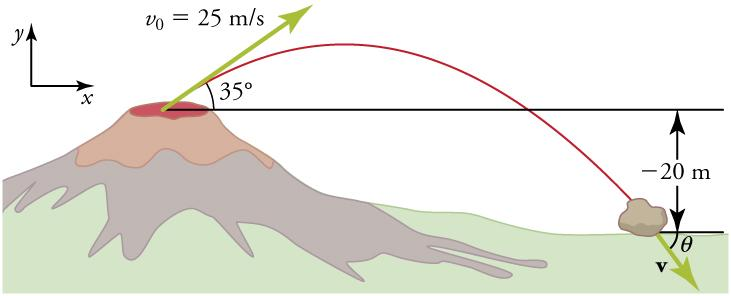
\includegraphics[width=0.5\linewidth]{2021-1/Imagenes/aux2/volcan.jpg}
    \caption*{Figura P2}
\end{figure}

\item Un cohete viaja verticalmente gracias a sus motores con una aceleración conocida $a_0$ hacia arriba, partiendo con velocidad nula. Al mismo instante en que parte el cohete y desde el mismo nivel, se dispara un proyectil con la intención de destruirlo en el aire. La separación horizontal cuando ambos objetos despegan es $L$, mientras que el ángulo inicial respecto a la horizontal del proyectil tiene un valor $\theta$. Calcule la rapidez inicial $v_0$ que posee el proyectil para que logre impactar el cohete

\begin{figure}[h!]
    \centering
    \begin{subfigure}[t]{0.4\textwidth}
        \centering
        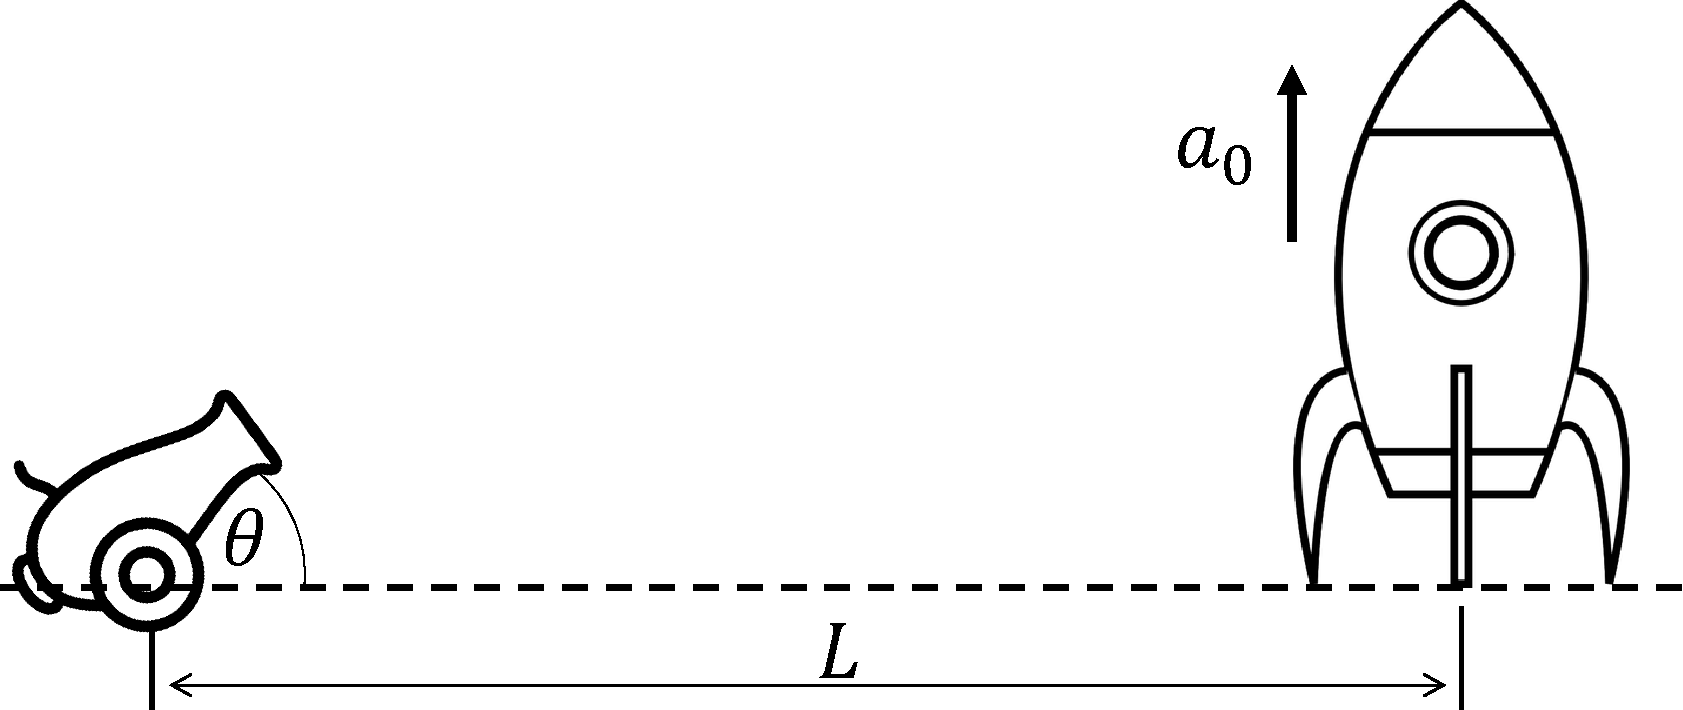
\includegraphics[width=0.8\linewidth]{2021-1/Imagenes/aux2/cohete-cannon.pdf}
        \caption*{Figura P3}
    \end{subfigure}
    \hspace{0.5cm}
    \begin{subfigure}[t]{0.4\textwidth}
        \centering
        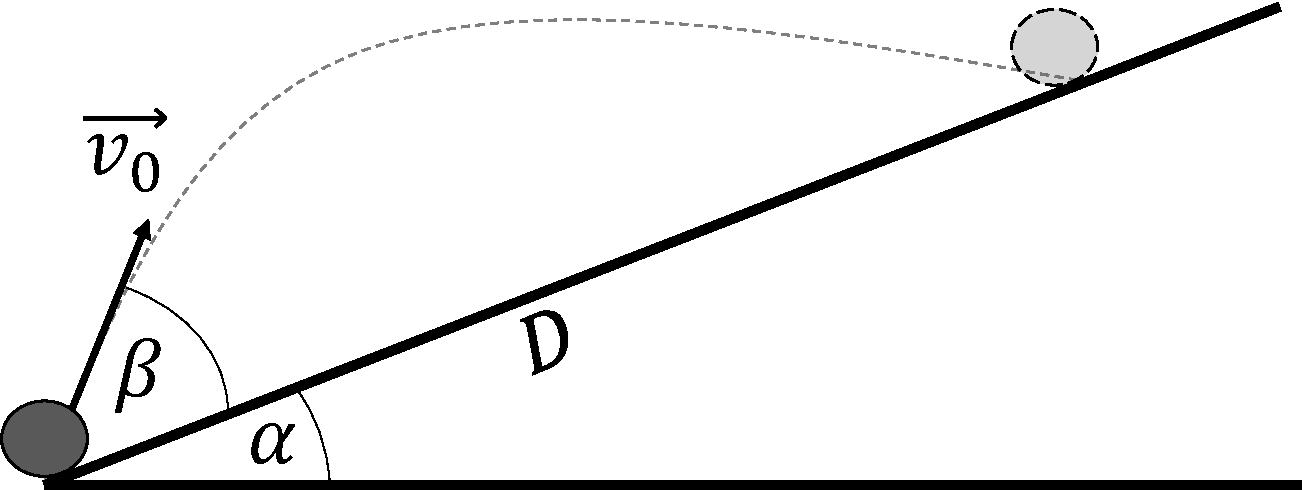
\includegraphics[width=0.9\linewidth]{2021-1/Imagenes/aux2/plano.pdf}
        \caption*{Figura P4}
    \end{subfigure}
\end{figure}

\item Un proyectil es lanzado desde un plano inclinado cuyo ángulo de inclinación con la horizontal es $\alpha$. Si el proyectil es lanzado con rapidez $v_0$ y con un ángulo de eyección $\beta$ con respecto al plano, calcule el alcance $D$ del proyectil a lo largo del plano.



\end{enumerate}
\end{document}